\section{Конструкторская часть}

\subsection{Разработка алгоритма поиска общего названия ВУЗа}

Поскольку количество анализируемых ВУЗов составляет несколько сотен, сбор данных должен производиться в автоматизированном режиме.

В процессе анализа статистических данных было обнаружено, что именования ВУЗов на аналитических ресурсах различны, что затрудняет их объединение, поскольку название ВУЗа в данном случае является его уникальным идентификатором. 

Одним из вариантов решения данной задачи является отправка двух запросов в сеть Интернет, где в  качестве параметра поиска передавать название ВУЗа с информационного источника. Таким образом, будут получены соответствия для двух различных названий ВУЗов и одного унифицированного, с помощью которого можно производить объединение данных.

\subsection{Разработка алгоритма приведения данных к официальному перечню направлений подготовки высшего образования}

В данных об укрупнённых группах специальностей и направлений, полученных с мониторинга качества приёма в ВУЗы\cite{miccedu}, существует допущение — указаны неофициальные укрупнённые группы, составленные самим мониторингом из официальных групп. Для решения данной задачи необходимо выделить таблицу, в которой будет указано, какую долю имеет официальная группа, в неофициальной. С помощью данной таблицы можно пересчитать количество бюджетных мест по формуле 

\begin{equation}
N_{budget} = \sum P_{i} k_{i},
\end{equation}
\begin{tabular}{llll}
    где & $N_{budget}$ & {---} & количество бюджетных мест в официальной группе; \\
    \addlinespace
    & $P_{i}$ & {---} & \begin{tabular}[t]{@{}l@{}}количество мест в i-ой неофициальной группе;\end{tabular} \\
    \addlinespace
    & $k_{i}$ & {---} & \begin{tabular}[t]{@{}l@{}} i-я доля официальной группы в неофициальной.\end{tabular}
\end{tabular} \\

Средний балл в каждой группе ВУЗа из информационно-аналитических материалов по следующей формуле

\begin{equation}
B_{aver.score} = \frac{\sum P_{i} k_{i} B_{i}}{N_{budget}},
\end{equation}
\begin{tabular}{llll}
    где & $B_{aver.score}$ & {---} & средний балл в официальной группе; \\
    \addlinespace
    & $B_{i}$ & {---} & \begin{tabular}[t]{@{}l@{}}средний балл в i-ой неофициальной группе.\end{tabular} \\
\end{tabular} \\

Последним этапом приведения будет масштабирование значений количества бюджетных мест и среднего балла в группе. Его необходимо проводить, если верно следующее:

\begin{equation}
N_{offical} \neq  N_{unoffical},
\end{equation}
\begin{tabular}{llll}
    где & $N_{offical}$ & {---} & сумма бюджетных мест всех  официальных групп ВУЗа; \\
    \addlinespace
    & $N_{unoffical}$ & {---} & \begin{tabular}[t]{@{}l@{}}сумма бюджетных мест всех  неофициальных групп ВУЗа.\end{tabular} \\
\end{tabular} \\

В данном случае необходимо пересчитать количество бюджетных в каждой группе по описанной выше формуле:

\begin{equation}
N_{budget} = \mu \sum P_{i} k_{i},
\end{equation}
\begin{tabular}{llll}
    где & $\mu = \frac{N_{offical}}{N_{unoffical}}$ \\
\end{tabular} \\


Формула для пересчёта среднего балла остается без изменений.

\subsection{Характеристики агента}

В данной задаче агентами являются абитуриенты – сущности, обладающие активностью и характеристиками.

Базовыми характеристиками абитуриента являются:

\begin{itemize}[leftmargin=1.6\parindent]
	\item[---] уникальный идетификатора абитуриента;
	\item[---] возможность смены региона;
	\item[---] результаты сдачи ЕГЭ;
	\item[---] интересующие УГСН, определяющиеся по сданным ЕГЭ.

\end{itemize}


\subsection{Генерация популяции агентов}



\subsection{Модель поведения агента}

Каждый абитуриент оценивает свою ситуацию, анализируя свое положение в конкурсном списке (отсортированном по сумме баллов ЕГЭ) и по количеству доступных бюджетных мест на данный УГСН. Если он не попадает в доступные места, то принимется решение о полной смене текущего ВУЗа со всеми заявлениями в нем или о поиске другого ВУЗа, в который можно положить заявление на такой же УГСН.

Оценивание ситуаций производится до тех пор, пока можно подавать новые заявления. Затем абитуриент должен положить оригинал аттестата к одному из своих заявлений. Искомое заявление выбирается исходя из престижности ВУЗа – абитуриенты стремятся попасть в наиболее престижные места. Если выбор проиводится внутри одного ВУЗа на разных УГСН, то сравниваются величины престижности данных УГСН. 

На этапе выбора заявления для подачи оригинала аттестата возможна ситуация, когда абитуриент не имеет ни одного заявления с копией аттестата, соответственно он не может претендовать на возможность обучения в ВУЗе.

\subsection{Разработка метод прогнозирования итогов приема в ВУЗы}

Ниже представлена IDEF0-диаграмма разрабатываемого метода на рисунке  \ref{A-0}.

\begin{figure}[hbtp]
	\centering
	\includegraphics[scale=0.8]{idef0/01\_A-0.pdf}
	\caption{IDEF0 диаграмма ветка A-0}
	\label{A-0}
\end{figure}

Разрабатываемый метод прогнозирования состоит из четырех этапов:

\begin{itemize}[leftmargin=1.6\parindent]
	\item[---] базовое распределение абитуриентов по ВУЗам на основе проходного балла прошлого года;
	\item[---] перераспределение агентами поданных заявлений для поиска УГСН, на который имеются шансы пройти по бюджетным местам в текущий момент;
	\item[---] подача оригинала аттестата к своему заявлению, по результатам сравнения престижности ВУЗов и их УГСН;
	\item[---] анализ полученных результатов.
\end{itemize}

\begin{figure}[hbtp]
	\centering
	\includegraphics[scale=0.8]{idef0/02\_A0.pdf}
	\caption{IDEF0 диаграмма ветка A0}
	\label{A0}
\end{figure}

Настройки конфигурации включают в себя поля:

\begin{itemize}[leftmargin=1.6\parindent]
	\item[---] год проведения моделирования;
	\item[---] количество абитуриентов, участвующих в моделировании;
	\item[---] значения долей четырех категорий агентов;
	\item[---] диапазон баллов ЕГЭ, которые будут заданы агентам каждой категории;
	\item[---] минимальные баллы ЕГЭ по каждому предмету;
	\item[---] длительность этапа перераспределения заявлений с копиями аттестатов;
	\item[---] длительность этапа поиска заявления на УГСН для оригинала аттестата.

\end{itemize}

Первым этапом моделирования явлется базовое распределение абитуриентов по УГСН в ВУЗах на основе среднего балла по УГСН в прошлом году. Абитуриенты просматривают ВУЗы, начиная с самого престижного, проверяют наличие интересующего УГСН, какие результаты ЕГЭ необходимы для подачи заявления, сравнивают со своими результатами (средним баллом по предметам, необходимым для поступления на данный УГСН) и кладут копию аттестата к заявлению.

Второй этап моделирования представлен в виде схемы алгоритма поиска подходящих УГСН на рисунке \ref{scheme:find}

\begin{figure}[hbtp]
	\centering
	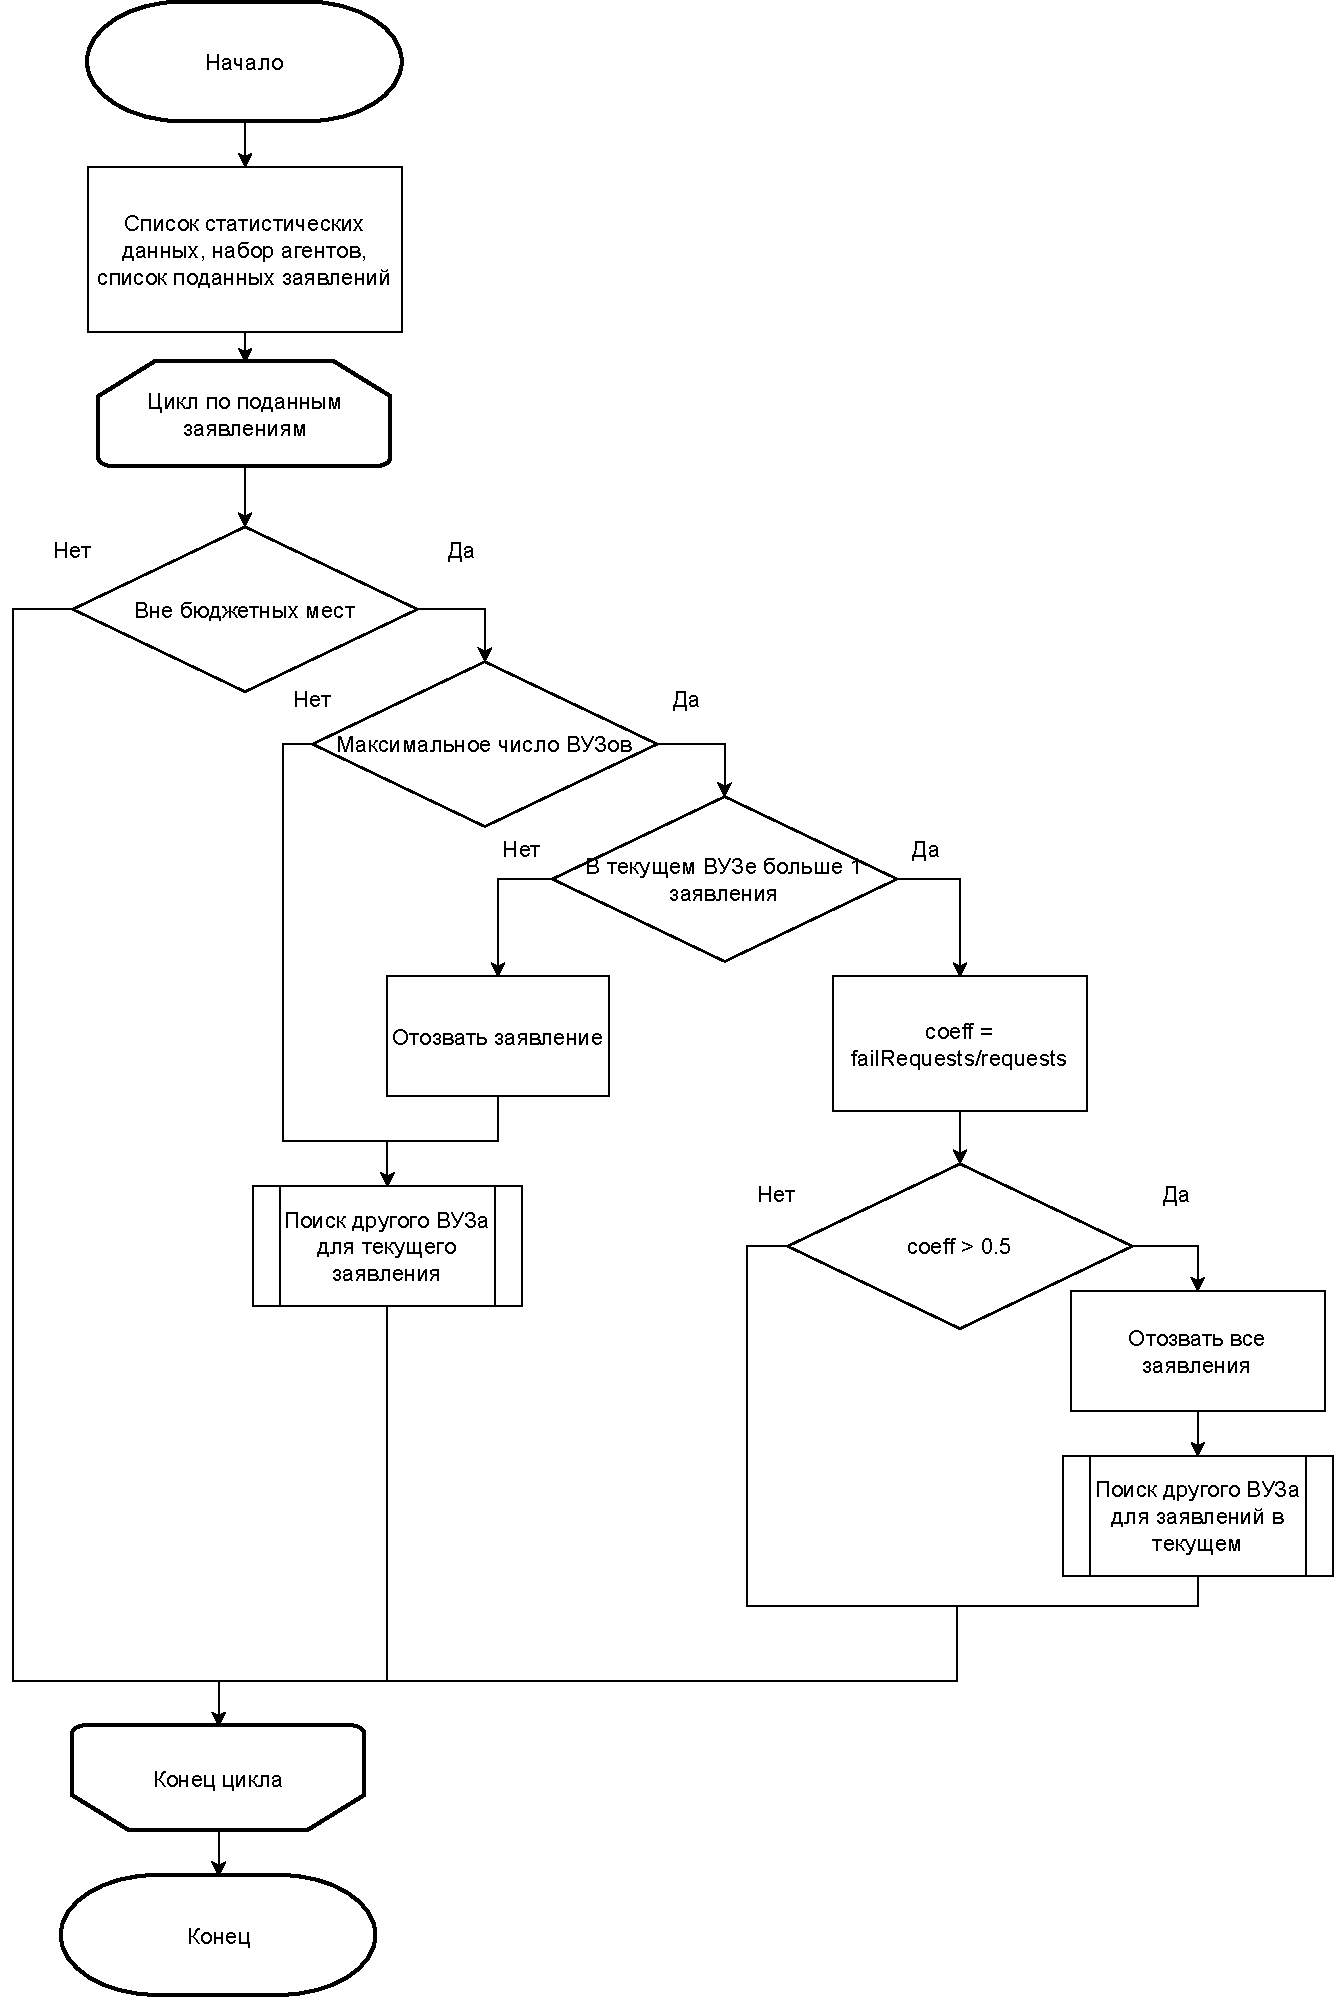
\includegraphics[scale=0.6]{idef0/find.pdf}
	\caption{Схема алгоритма поиска подохящего УГСН}
	\label{scheme:find}
\end{figure}


Третий этап – подача оригинала аттестата к свою заявлению и зачисления. Студенты, не имеющие заявлений ни в каком ВУЗе не рассматриваются. Анализируем каждое заявление абитуриента, проходит ли он в текущий момент по бюджетным местам среди других абитуриентов с оригиналами аттестатов. Отмечаем данную заявку как лучшую, если абитуриент проходит на нее и она лучше предыдущего выбора. Сравнение текущего и предыдущего выбора производится на основе престижности ВУЗа, если сравниваются УГСН в разных ВУЗах и престижности УГСН, если сравнение производится внутри одного ВУЗа. Зачисление на доступные бюджетные места абитуриентов с наиболее выскоими баллами в конкурсном списке.

Завершающий этап - анализ сложившейся ситуации в конкурсном списке каждого УГСН, вычисление минимального, максимального, среднего балла по данному УГСН и ВУЗу в целом и сравнение результата моделирования с итогами приема абитуриентов предыдущего года.





















\pagebreak